\chapter{Energy Calibration}\label{ch:energyCalibration}

Scope of the energy calibration is to identify the factors which convert the charge collected (dQ) to energy deposited in the chamber (dE). As described in section \ref{sec:SignalProc}, this is a multi-step procedure. In LArIAT, we first correct the raw charge by the electronic noise on the considered wire \cite{LArIATdqdx}, then by the electron lifetime \cite{LArIATLifeTime},  and then by the recombination using the ArgoNeut recombination values. Lastly, we apply overall calibration of the energy, i.e. we determine the ``calorimetry constants" using the procedure described in this section.


We independently determine  the calorimetry constants for Data and Monte Carlo in the LArIAT Run-II Data samples using  a parametrization of the stopping power (a.k.a. energy deposited per unit length, $dE/dX$)  as a function of momentum. This is done by comparing the stopping power measured on reconstructed quantities against the Bethe-Bloch theoretical prediction for various particle species (see Equation \ref{eq:BB}).  We obtain the theoretical expectation for the $dE/dX$ most probable value of pions ($\pi$), muons ($\mu$), kaons ($K$), and protons ($p$) in the momentum range most relevant for LArIAT (Figure \ref{fig:PDGEnergyLossArgon}) using the tables provided by the Particle Data Group \cite{Patrignani:2016xqp} for liquid argon \cite{PDG-Argon}.

The basic idea of this calibration technique is to utilize a sample of beamline events with known particle species and momentum to measure the $dE/dX$ of the corresponding tracks in the TPC. In particular, we decided to use positive pions as calibration sample and samples from all the other particle species as cross check. Once the $dE/dX$ of the positive pion sample  has been measured at various momenta, we tune to calorimetry constants within the reconstruction software to align the measured values to match the theoretical ones found in Figure \ref{fig:PDGEnergyLossArgon}. 

In data, we start by selecting a sample of beamline positive pion beamline candidates without any restriction on their measured momentum\footnote{it should be noted that some muon and position contamination is present in the $\pi^+$ sample}.
We then apply the WC2TPC match and subtract the energy loss upstream to the TPC front face, determining the momentum at the TPC front face. For each surviving pion candidate,  we measure the $dE/dx$ at each of the first 12 spacepoints associated the 3D reconstructed track, corresponding to a $\sim$ 5 cm portion. These $dE/dX$ measurements are then put into a histogram that corresponds to measured momentum of the track. The $dE/dX$ histograms are sampled every 50 MeV/c in momentum (e.g. 150~MeV/c $< P <$ 200~MeV/c, 200~MeV/c $< P <$ 250/c~MeV, etc...).   This process of selecting, sampling, and recording the $dE/dX$ for various momentum bins is repeated over the entire sample of events, allowing us to collect sufficient statistic in most of the momentum bins between 150~MeV/c and 1100~MeV/c. On average, pions and muons only lose $\sim$10 MeV in this 5~cm section of the track and protons lose $\sim$20 MeV. Thus choosing 50 MeV/c size bins for our histograms covers the energy spread within those bins due to energy loss from ionization for all the particle species identifiable in the beamline. 
Each 50 MeV/c momentum binned $dE/dX$ histogram is now fit with a simple Landau function. The most probable value (MPV) and the associated error on the MPV from the fit are extracted and plotted against the theoretical prediction Figure \ref{fig:PDGEnergyLossArgon}. Depending on the outcome of the data-prediction comparison, we modify the calorimetry constants and we repeat the procedure until a qualitative agreement is achieved.  We perform this  tuning for the collection and induction plane separately. 
As a cross check to the calorimetry constants determined using the positive pions, we lock the constants and  plot the $dE/dx$ versus momentum distribution of all the other particle species identifiable in the beamline data ($\pi/\mu/e$, K , p, in both polarities) against the corresponding Beth-Bloch prediction. The agreement between data from the other particle species and the predictions is the expected result of this cross check.
The results of the tuning and cross check for Run-II data on the collection plane is shown in Figure \ref{fig:BBandData}  negative polarity data on top, positive polarity data on the bottom.

In MC, we simulate the corresponding positive pion sample with the DDMC (see section \ref{sec:DDMC}) and follow the same steps as in data. More details on the calorimetry tuning can be found in \cite{LArIATCalo}.

After the calibration is done separately on data and MC, we can compare the resulting dE/dX distributions; this is done for the set of pion beamline candidates and pion MC on the left side of Figure \ref{fig:dedx}. On the right side of the same figure, we report the data-MC comparison for the kaon sample used in the cross section. The distributions are fitted with simple Landau functions. As expected, the Landau MPV for data  is consistent with the MC MPV for both pions and kaons. For both the pion and the kaon case, the width of the Landau is a bit wider in data than in MC; this difference might be due to an underestimate of the electronic noise in the MC simulation.


\begin{figure}[htb]
\centering
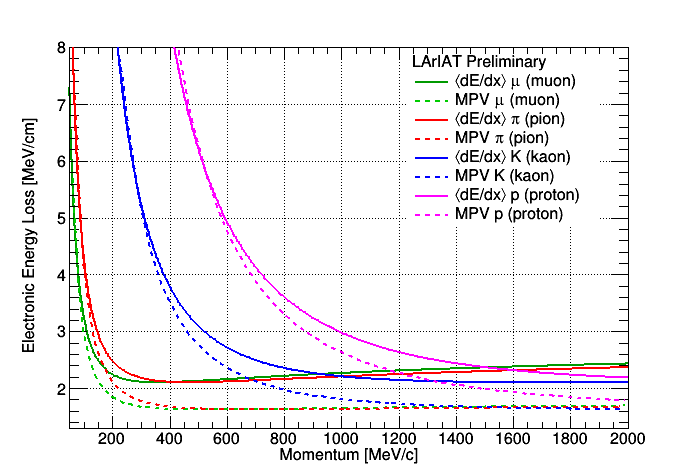
\includegraphics[width=0.50\textwidth]{Chapter-5/Images/dEdXvsMomentumTemplate.png}
\caption{Stopping power for pions, muons, kaons, and protons in liquid argon over the momentum range most relvant for LArIAT according to the Beth-Bloch equation. The solid lines represent the prediction for the mean energy $dE/dX$, while the dashed lines are the predictions for the MPV.}
\label{fig:PDGEnergyLossArgon}
\end{figure}


\begin{figure}[htb]
\centering
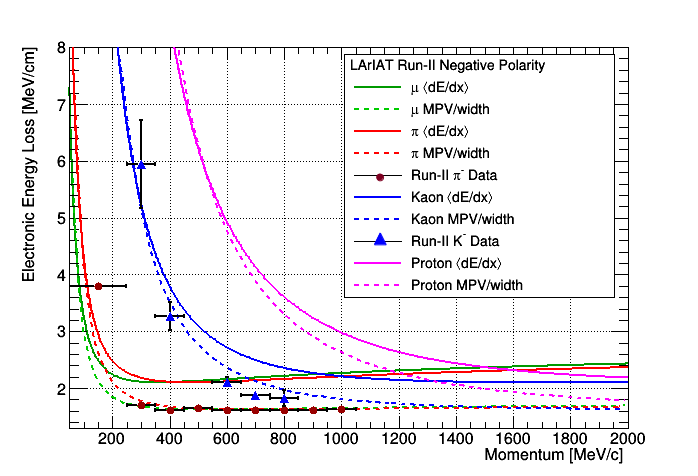
\includegraphics[width=0.48\textwidth]{Chapter-5/Images/RunIINegTotaldEdXvsMomentum.png}
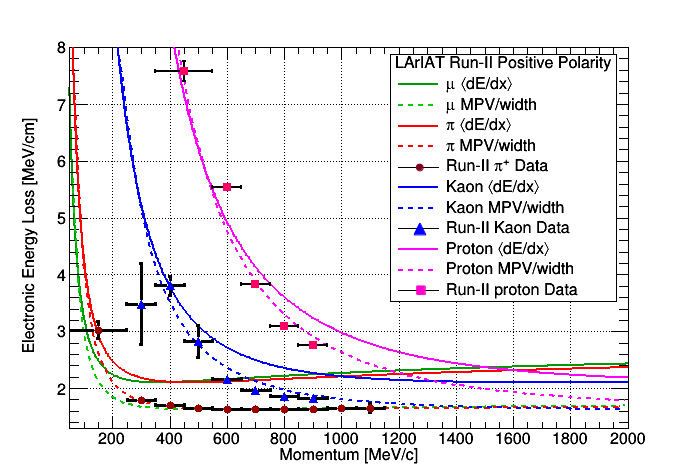
\includegraphics[width=0.48\textwidth]{Chapter-5/Images/RunIIPosTotaldEdXvsMomentum.png}
\caption{Stopping power versus Momentum for Run-II negative (top) and positive (bottom) polarity data. We achieve the agreement between the Bethe-Bloch predictions and the distribution obtained with of the positive pions (top plot, red dots) by tuning the calorimetry constants. Once the calorimetry constants are locked in, the agreement between the other particle species and the Bethe-Bloch predictions follows naturally.}
\label{fig:BBandData}
\end{figure}


\begin{figure}[htb]
\centering
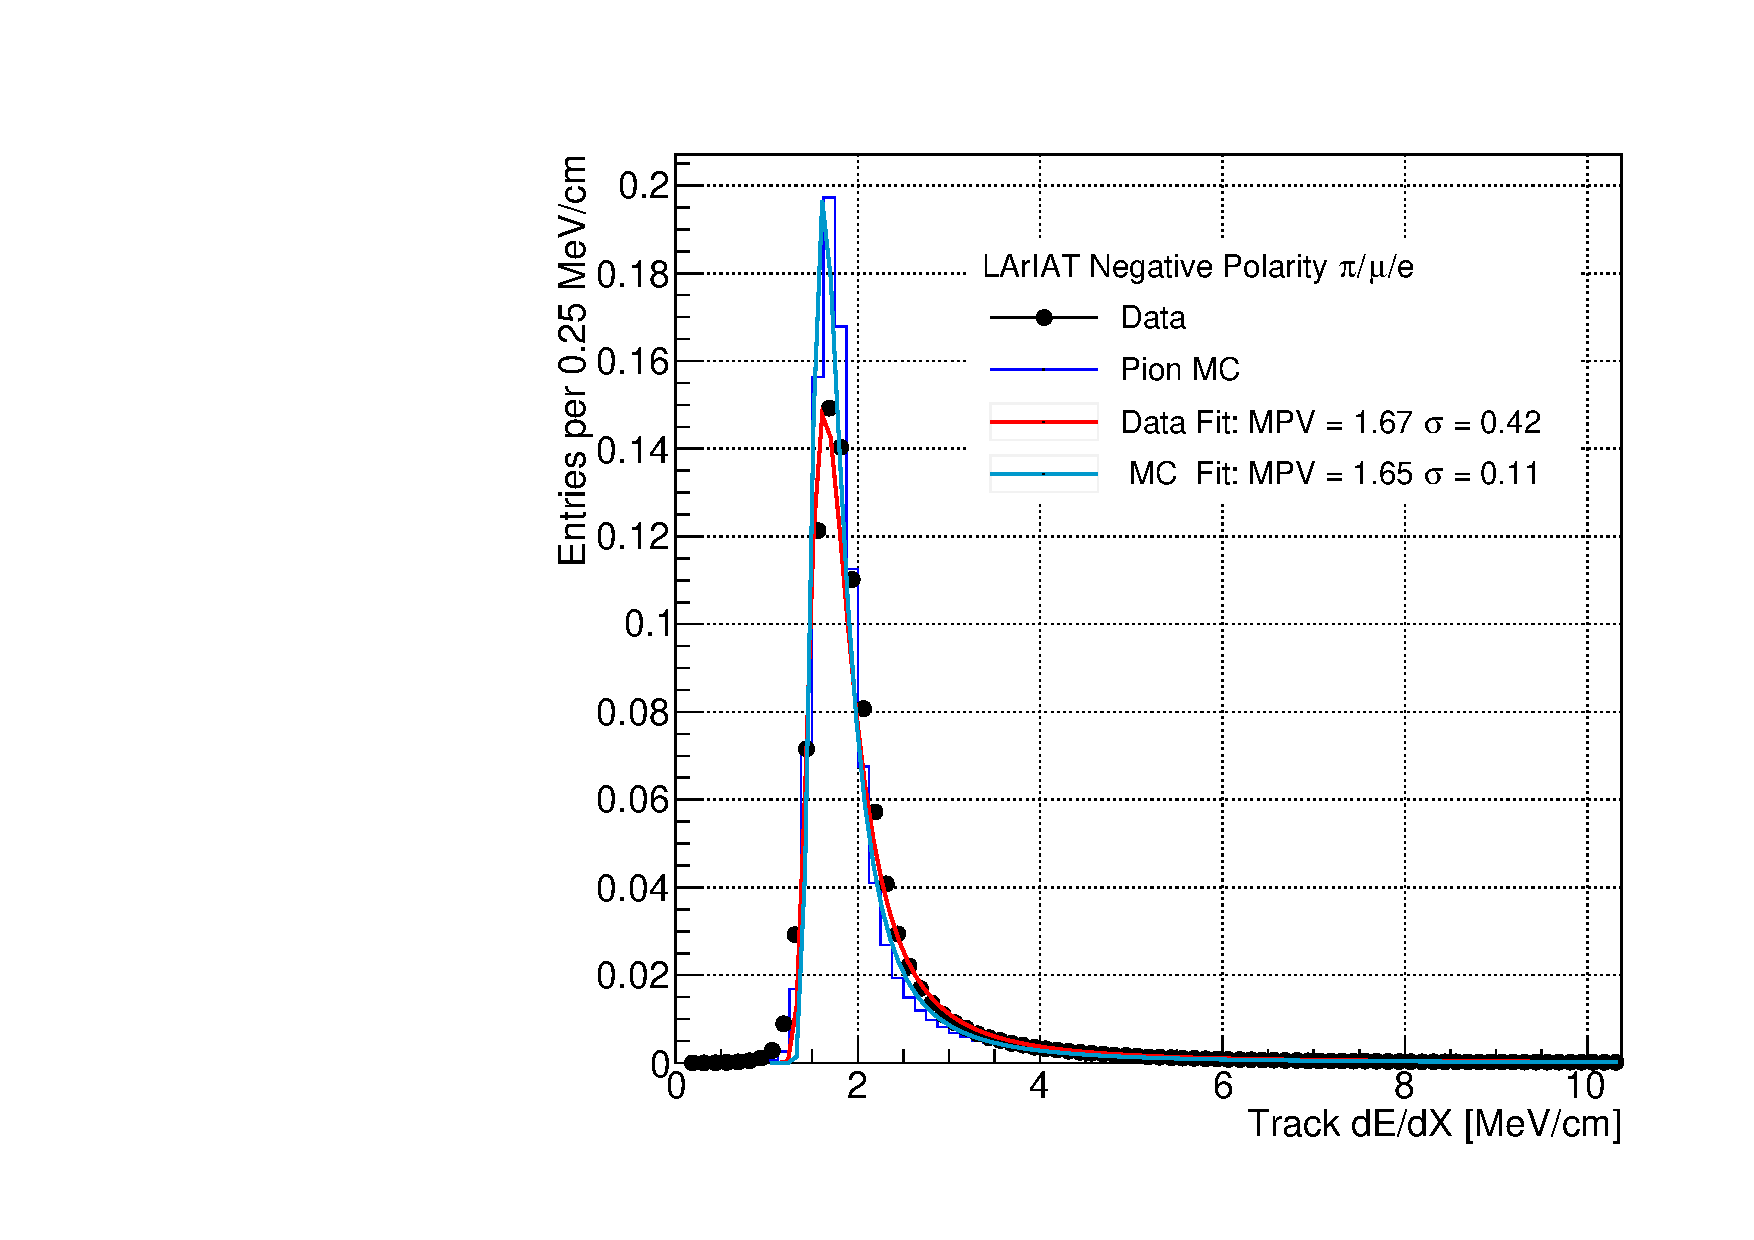
\includegraphics[width=0.48\textwidth]{AppendixC-EnergyCalibration/dEdXPions.pdf}
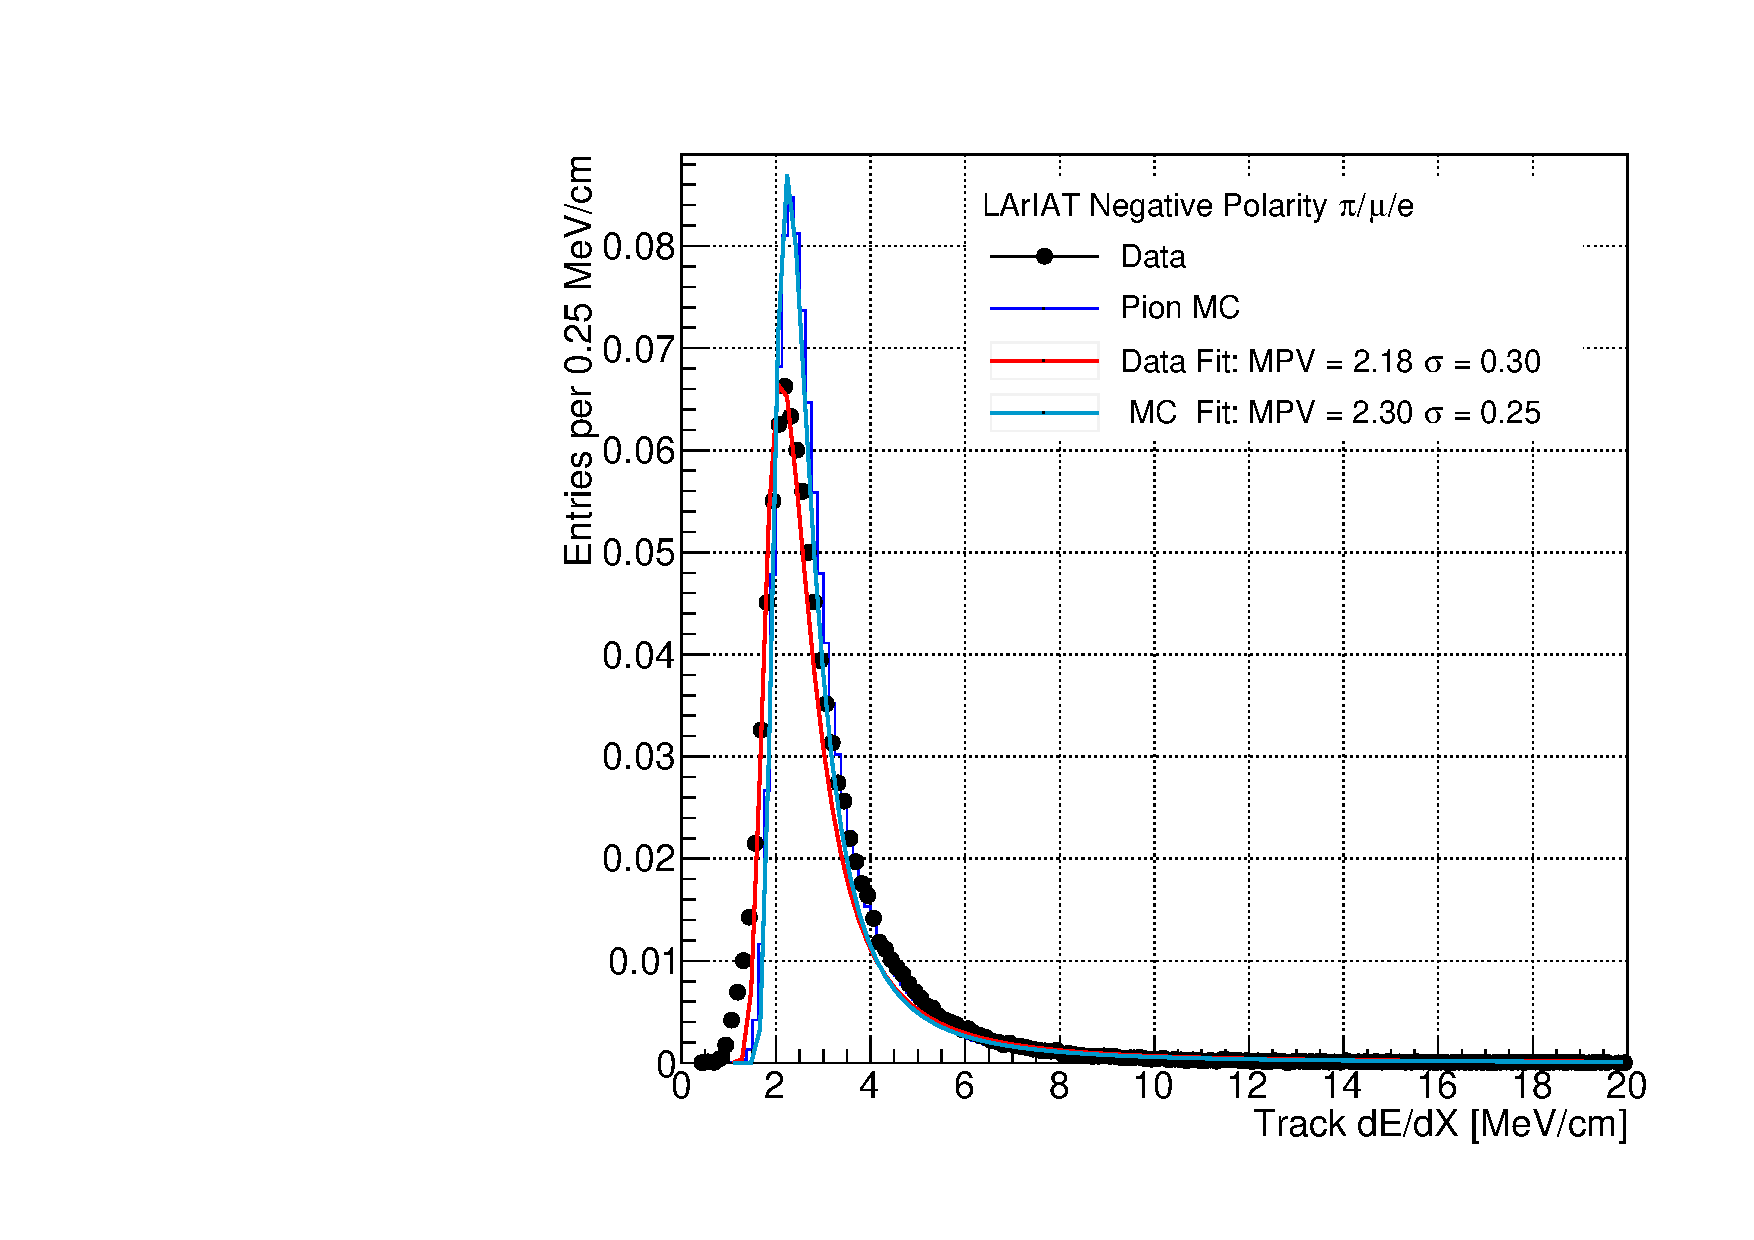
\includegraphics[width=0.48\textwidth]{AppendixC-EnergyCalibration/dEdXKaons.pdf}
\caption{\emph{Left:} dE/dx distribution for $\pi^-/\mu^-/e^-$ data (black) and Pion MC (blue). The Landau fit for data is shown in red, the one for MC in teal.\emph{Right:} dE/dx distribution for $K^+$ data (black) and Kaon MC (blue). The Landau fit for data is shown in red, the one for MC in teal. All the distributions are area normalized.}
\label{fig:dedx}
\end{figure}


%\begin{figure}[htb]
%\centering
%\includegraphics[width=0.50\textwidth]{images/CalibrationExample.png}
%\caption{Illustration of the calibration technique. Here we depict a 325 MeV wire chamber track (shown in green) which enters the TPC (taking into account the energy loss from the upstream material) and we sample the first 12 spacepoints (shown in teal) to extract the dE/dX distribution which is fit with a Landau.}
%\label{fig:CalibrationExample}
%\end{figure}



